%%%%%%%%%%%%%%%%%%%%%%%%%%%%%%%%%%%%%%%%%%%%%%%%%%%%%%%%%%%%%%%%%%%%%%%%%%%%%%%%
%%%%%%%%%%%%%%%%%%%%%%%%%%%%%%%%%%%%%%%%%%%%%%%%%%%%%%%%%%%%%%%%%%%%%%%%%%%%%%%%
\documentclass[addpoints,12pt,solution]{exam}
\printanswers
\usepackage{amsmath,amssymb}
\usepackage{comment}
\usepackage{graphicx}
\usepackage{ulem}
\usepackage{paralist}
\usepackage{psfrag}
\usepackage{fullpage}
\usepackage{fancybox}
\usepackage{ifthen}
\usepackage{enumitem}
\usepackage{hyperref}
\usepackage{marvosym}
\usepackage{amsmath,amsthm}
\DeclareMathOperator*{\argmax}{arg\,max}
\DeclareMathOperator*{\argmin}{arg\,min}
\usepackage[ruled,vlined,noresetcount]{algorithm2e}
\usepackage{enumitem}
\marksnotpoints
\usepackage{hyperref}
\hypersetup{
    colorlinks=true,
    linkcolor=blue,
    filecolor=magenta,      
    urlcolor=cyan,
    pdftitle={Overleaf Example},
    pdfpagemode=FullScreen,
    }

\newcommand{\bw}{\textbf{w}}
\newcommand{\bq}{\textbf{q}}
\newcommand{\bp}{\textbf{p}}
\newcommand{\bP}{\textbf{P}}
\newcommand{\bQ}{\textbf{Q}}
\newcommand{\bA}{\textbf{A}}
\newcommand{\bR}{\mathbb{R}}
\newcommand{\bI}{\mathbf{I}}

\begin{document}


\hrule
\vspace{1mm}
\noindent 
\begin{center}
{\Large CS5691: PRML Assignment \#2} \\


\end{center}
\noindent {\small \textbf{Instructor} : Prof. B. Ravindran } \\ 
\noindent \small{\textbf{Topics:} ANN,Ensemble Method,Kernel and SVM. \hfill \textbf{Deadline:} 12th November 2021} \\


%%%%%%%%%%%%%%%%%%%%%%%%%%%%%%%%%%%%%%%%%%%%%%%%%%%%%%%%%%%%%%%%
% Enter name and roll number here
\noindent {\bf Teammate 1:} (your name here) \hfill {\bf Roll number:} CS21YZZZ \\
\noindent {\bf Teammate 2:} (your name here) \hfill {\bf Roll number:} CS21YZZZ \\
%%%%%%%%%%%%%%%%%%%%%%%%%%%%%%%%%%%%%%%%%%%%%%%%%%%%%%%%%%%%%%%%%%
\vspace{2mm}
\hrule

{\small

\begin{itemize}\itemsep0mm

\item This assignment has to be completed in teams of 2. Collaborations outside the team are strictly prohibited.

\item Be precise with your explanations. Unnecessary verbosity will be penalized.

\item Check the Moodle discussion forums regularly for updates regarding the assignment.

\item Type your solutions in the provided \LaTeX ~template file.


\item We highly recommend using \texttt{Python 3.6+} and standard libraries like \texttt{numpy, Matplotlib, pandas}. You can choose to use your favourite programming language however the TAs will only be able to assist you with doubts related to Python. 

\item You are supposed to write your own algorithms, any library functions which implement these directly are strictly off the table. Using them will result in a straight zero on coding questions, \texttt{import} wisely!

\item \textbf{Please start early and clear all doubts ASAP.}

\item Please note that the TAs will \textbf{only} clarify doubts regarding problem statements. The TAs won't discuss any prospective solution or verify your solution or give hints.  

\item Post your doubt only on Moodle so everyone is on the same page.

\item Posting doubts on Moodle that reveals the answer or gives hints may lead to penalty

\item \textbf{Only one team member will submit the solution} 

\item For coding questions paste the link to your Colab Notebook of your code in the \LaTeX ~solutions file as well as embed the result figures in your \LaTeX ~solutions. Make sure no one other than TAs have access to the notebook. And do not delete the outputs from notebook before final submission . Any update made to notebook after deadline will result in standard late submission penalty.
\item Late submission per day will attract a penalty of 10 percent of the total marks.

\end{itemize}
}

\hrule

\vspace{3mm}

%%%%%%%%%%%%%%%%%%%%%%%%%%%%%%%%%%%%%%%%%%%%%%%%%%%%%%%%%%%%%%%%%%%%%%%%%%%%%%%
%%%%%%%%%%%%%%%%%%%%%%%%%%%%%%% START HERE %%%%%%%%%%%%%%%%%%%%%%%%%%%%%%%%%%%%
\begin{questions}

%%%%%%%%%%%%%%%%%%%%%%%%%%%%%%%%%%%%%%%%%%%%%%%%%%%%%%%%%

\question \textbf{[ANN]} In this Question, you will code a single layer ANN with Sigmoid Activation function and appropriate loss function from scratch. Train the ANN for the \href{https://drive.google.com/drive/folders/1sNvKGEguK_Se7ktKm68ItIDVO6QDVe6w?usp=sharing}{Dataset1} and \href{https://drive.google.com/drive/folders/1Vpby8jKYi72rRzzM51sSqB78PS0Tb6Bl?usp=sharing}{Dataset2}  


\textbf{NOTE: Test Data should not be used for training.}
\smallbreak
\textbf{NOTE 2: You need to code from scratch.}


\begin{parts}

\part[1] Plot the training Data for Dataset1 and Dataset2.
\begin{solution}

\end{solution}

\part[1]\textbf{For data set 1} : (1) Write the number of nodes in the hidden layer and learning rate used (2) Plot Test Data and prediction on Test Data in the same graph with different colors and appropriate legend.

\begin{solution}

\end{solution}

\part[1]\textbf{For data set 2} : (1)  Write the number of nodes in the hidden layer and learning rate used (2) Plot Test Data and prediction on Test Data in the same graph with different colors and appropriate legend.

\begin{solution}

\end{solution}
\part[1]For each Dataset write average training Loss and average Test Loss.

\begin{solution}

\end{solution}
\part[1]What Loss function did you use and why?


\begin{solution}

\end{solution}
\part[3]Paste the link to your Colab Notebook of your code. Make sure that your notebook is private and give access to all the TAs. Your Notebook must contain all the codes that you used to generate the above results.\textbf{ Note : } Do not delete the outputs.
\begin{solution}

\end{solution}
\end{parts}

%%%%%%%%%%%%%%%%%%%%%%%%%%%%%%%%%%%%%%%%%%%%%%%%%%%%%%%%%

\question \textbf{[AdaBoost]} In this question, you will code  the AdaBoost algorithm. Follow the instructions in this \href{https://drive.google.com/file/d/1EXxgwze28jnrkafl_7F99AJ7uD9gdIMI/view?usp=sharing}{Jupyter Notebook} for this question. Find the dataset for the question \href{https://drive.google.com/drive/folders/1V52vjD8PHoLikP8sfAPi7hWABRwJ_7HQ?usp=sharing}{here}.

\textbf{NOTE: Test data should not be used for training.}
\smallbreak \textbf{NOTE 2: You need to code from scratch. } You can use the starter notebook though :) . Make a copy of it in your drive and start.
\begin{parts}

\part[1] Plot the training data.
\begin{solution}

\end{solution}

\part[1]\textbf{For training with k=5} : (1)  Plot the learnt decision surface. (2) Write down the test accuracy.

\begin{solution}

\end{solution}

\part[1]\textbf{For training with k=100} : (1)  Plot the learnt decision surface. (2) Write down the test accuracy.

\begin{solution}

\end{solution}

\part[3]Paste the link to your Colab Notebook of your code. Make sure that your notebook is private and give access to all the TAs. Your notebook must contain all the codes that you used to generate the above results. \textbf{Note : } Do not delete the outputs.
\begin{solution} 

\end{solution}
\end{parts}

%%%%%%%%%%%%%%%%%%%%%%%%%%%%%%%%%%%%%%%%%%%%%%%%%%%%%%%%%%

\question \textbf{[Kernel]} Consider $Dataset\_Kernel\_Train.npy$ and $Dataset\_Kernel\_Test.npy$ for this question. Each row in the above matrices corresponds to a labelled data point where the first two entries correspond to its $x$ and $y$ co-ordinate, and the third entry $\in \{-1,1\}$ indicates the class to which it belongs.
Find the dataset for the question \href{https://drive.google.com/drive/folders/1rLcNySI1dUEvlt9eobrinp8cuoVrE1u9?usp=sharing}{here}.
\textbf{NOTE: Test data should not be used for training.}


\begin{parts}
\part[1] Plot the training data points and indicate by different colours the points belonging to the different classes. Is the data linearly separable?
\begin{solution}


\end{solution}

\part[1]  Using $sklearn.svm$ (read the documentation \href{https://scikit-learn.org/stable/modules/generated/sklearn.svm.SVC.html#}{here}), bulid a classifier that classifies the data points in the testing data set using the Radial Basis Function (RBF) kernel.How do you tune the involved hyperparameters?
\begin{solution}

\end{solution}

\part[1] Plot the separating curve and report the accuracy of prediction corresponding to the tuned hyperparameters.
\begin{solution}

\end{solution}
\part[3] Paste the link to your Colab Notebook of your code. Make sure that your notebook is private and give access to all the TAs. Your notebook must contain all the codes that you used to generate the above results. \textbf{Note : } Do not delete the outputs.
\begin{solution}

\end{solution}
\end{parts}
%%%%%%%%%%%%%%%%%%%%%%%%%%%%%%%%%%%%%%%%%%%%%%%%%%%%%%%%%%

\question[2] \textbf{[Ensemble of randomised algorithms]} Imagine we have an algorithm for solving some decision problem (\textit{e.g.}, is a given number $p$ a prime?). Suppose that the algorithm makes a decision at random and returns the correct answer with probability $\frac{1}{2} + \delta$, for some $\delta > 0$, which is just a bit better than a random guess. To improve the performance, we run the algorithm $N$ times and take the majority vote. Show that for any $\epsilon \in (0,1)$, the answer is correct with probability $1 - \epsilon$, as long as $N > (1/2)\delta^{-2} \ln (\epsilon^{-1})$.

\textit{Hint 1: Try to calculate the probability with which the answer is not correct i.e. when the majority votes are not correct.}

\textit{Hint 2: What value of $N$ will you require so that the above probability is less than $\epsilon$. Rearrange Inequalities :-)}

\begin{solution}
\end{solution}

\question[2] \textbf{[Boosting]} Consider an additive ensemble model of the form $f_m(\mathbf{x}) = \frac{1}{2} \sum_{l=1}^{m} \alpha_l y_l (\mathbf{x})$, where $y_l$'s are individual models and $\alpha_l$'s are weights. Show that the sequential minimization of the sum-of-squares error function for the above model trained in the style of boosting (i.e. $y_m$ is trained after accounting the weaknesses of $f_{m-1}$) simply involves fitting each new base classifier $y_m$ to the residual errors $t_n -f_{m-1}(\mathbf{x}_n)$ from previous model. 

\begin{solution}
\end{solution}

\question[2] \textbf{[Backpropagation]} We are trying to train the following chain like neural network with back-propagation. Assume that the transfer functions are sigmoid activation functions i.e. $g(x) = \frac{1}{1+e^{-x}}$. Let the input $x = 0.5$, the target output $y = 1$, all the weights are initially set to 1 and the bias for each node is -0.5.\\
    \begin{center}
        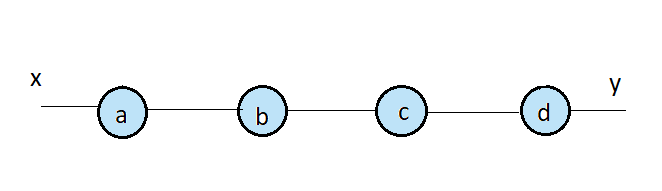
\includegraphics[scale=0.5]{bp.png}
    \end{center}
(a) Give an expression that compares the magnitudes of the gradient updates for weights ($\delta$) across the consecutive nodes.\\ 
(b) How does the magnitude of the gradient update vary across the network/chain as we move away from the output unit?

\begin{solution}
\end{solution}


\question[2] \textbf{[NN \& Activation Functions]} The following diagram represents a feed-forward network with two hidden layers. \\
\begin{center}
        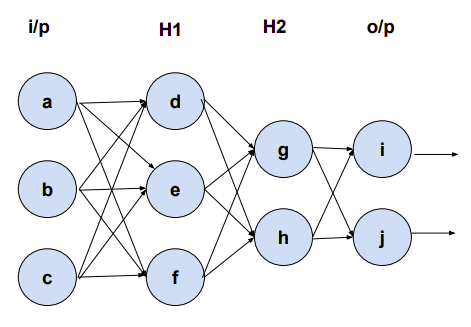
\includegraphics[scale=0.5]{NN.png}
\end{center}

A weight on connection between nodes $x$ and $y$ is denoted by $w_{xy},$ such as $w_{ad}$ is the weight on the connection between nodes a and d. The following table lists all the weights in the network: \\ 

\begin{center}
\begin{tabular}{|c|c|c|c|c |}
     $w_{ad} = 0.5$ & $w_{be} = -1.4$ & $w_{cf} = -1.25$ & $w_{eh} = -2$ & $w_{gj } = -1.5$\\
     $w_{ae} = 0.9 $ & $w_{bf} = 0.75$ & $w_{dg} = 1$ & $w_{fg} = 3$ & $w_{hi } = 0.5$\\
     $w_{af} = -2$ & $w_{cd} = 0$ & $w_{dh} = 3$ & $w_{fh} = 1.25$ & $w_{hj } = -0.25$\\
     $w_{bd} = 1.3$ & $w_{ce} = 0.3$ & $w_{eg} = 2.5$ & $w_{gi } = 2.5$& \\
\end{tabular}
\end{center}

Find the output of the network for the following input vectors: \\
$V_1 = [0.2, 1, 3]$, $V2 = [2.5, 3, 7]$, $V3 = [0.75, -2, 3]$

\begin{parts}
\part If \textit{sigmoid} activation function is used in both H1 \& H2 

\part If \textit{tanh} activation function is used in both H1 \& H2 

\part If \textit{sigmoid} activation is used in H1 and \textit{tanh} in H2 

\part If \textit{tanh} activation is used in H1 \& ReLU activation in H2
\end{parts}

Please provide all steps and explain the same. 

\begin{solution}
\end{solution}







\question[2] \textbf{[Decision Trees]} Consider a dataset with each data point $x \in \{0, 1\}^m$, i.e., $x$ is a binary valued feature vector with $m$ features, and the class label $y \in \{+1, −1\}$. Suppose the true classifier is a majority vote over the features, such that\\
$y = sign \Big(\sum_{i=1}^{m}\big( 2x_i - 1\big)\Big)$

where $x_i$ is the $i^{th}$ component of the feature vector. Suppose you build a binary decision tree with minimum depth, that is consistent with the data described above. What is the range of of number of leaves which  such a decision tree will have?
\begin{solution}
\end{solution}




%%%%%%%%%%%%%%%%%%%%%%%%%%%%%%%%%%% THE END %%%%%%%%%%%%%%%%%%%%%%%%%%%%%%%%%%%
\end{questions}
\end{document}